\documentclass[aspectratio=169,10pt]{beamer}

\begin{document}
	
	\begin{frame}{Model}
		\[
		\mathcal{H} = 
		\]
	\end{frame}
	
	
	\begin{frame}{Comparison}
		\begin{columns}
			\column{0.48\linewidth}
			\centering
			\begin{figure}
				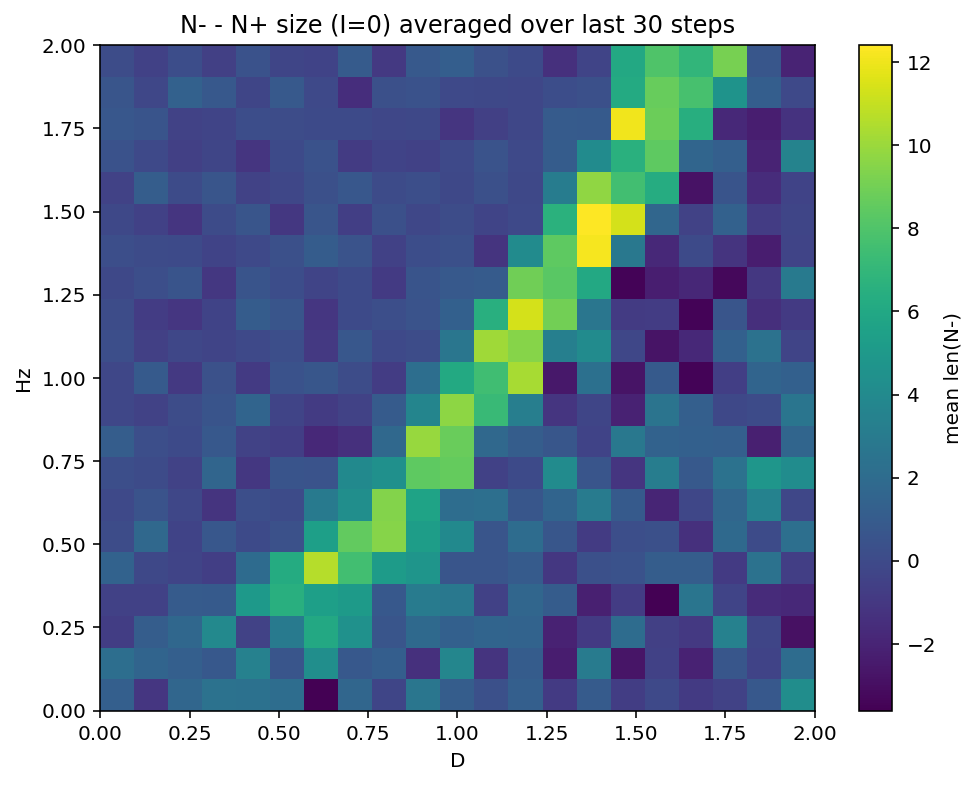
\includegraphics[width=\linewidth]{20x20 phase diagram.png}
			\end{figure}
			
			
			\column{0.48\linewidth}
			\centering
			
			\begin{figure}
				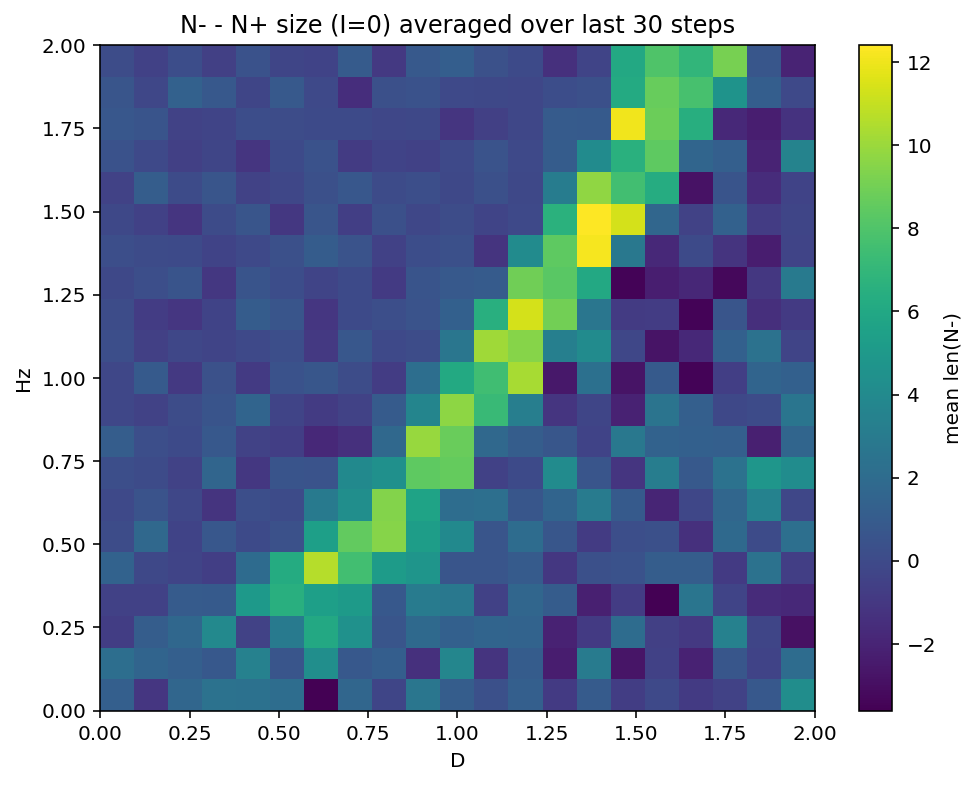
\includegraphics[width=\linewidth]{20x20 phase diagram.png}
			\end{figure}
			
		\end{columns}
		
	\end{frame}
	
	
	
	\begin{frame}{Detection}
		
		\begin{columns}
			\column{0.48\linewidth}
			\centering
			\begin{figure}
				
\includegraphics[width=\linewidth]{Lattice.png}
			\end{figure}
			
			
			\column{0.48\linewidth}
			\centering
			
			\begin{figure}
				
\includegraphics[width=\linewidth]{wrapping.png}
			\end{figure}
			
		\end{columns}
	\end{frame}
	
	
	
%	\begin{frame}{Detection}
%		
%		\begin{columns}
%			\column{0.48\linewidth}
%			\centering
%			\begin{figure}
%				\includegraphics[width=\linewidth]{2H 2D Lattice.png}
%			\end{figure}
%			
%			
%			\column{0.48\linewidth}
%			\centering
%			
%			\begin{figure}
%				\includegraphics[width=\linewidth]{2H 2D wrapping.png}
%			\end{figure}
%			
%		\end{columns}
%	\end{frame}
\end{document}